\documentclass{beamer}
\usepackage{graphicx}
\usepackage{mathtools}
\usepackage{tikz}
\usetikzlibrary{matrix,chains,positioning,decorations.pathreplacing,arrows}

\title{Movie Recommendations Using Low-dimensional Codes and User Specified Feature Relevance}
\author{Chris Curro, David Katz, Harrison Zhao} 
\date{May 2015}

\setbeamertemplate{itemize items}[circle]

\begin{document}

\begin{frame}
\titlepage
\end{frame}

\begin{frame}{Goal}
% An approach to generating a rich low-dimensional latent space capable of
% producing high quality movie recommendations based on a nearest neighbors
% where the queried sample is determined by user input.
\begin{itemize}
\item Rich low-dimensional latent space
\item High quality movie recomendations based on nearest neighbors
\item User input on the reocomendation
\end{itemize}
\end{frame}

\begin{frame}{Dataset}
Tag Genome dataset provied by grouplens
\begin{itemize}
\item 10,000 movies
\item 1,000 tags
\end{itemize}
\end{frame}

\begin{frame}{Approach}
\begin{itemize}
\item Autoencoders for nonlinear PCA
\item Nearest neighbors with weighted features
\end{itemize}
\end{frame}

\begin{frame}{Autoencoders}
\begin{equation}
\mathbf{y} = f\left(W\mathbf{x} + \mathbf{b}\right)
\end{equation}
\begin{center}
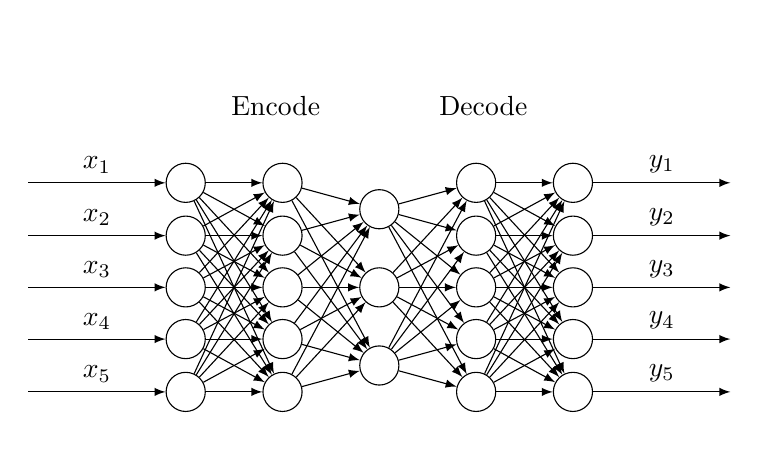
\begin{tikzpicture}[
plain/.style={
  draw=none,
  fill=none,
  },
net/.style={
  matrix of nodes,
  nodes={
    draw,
    circle,
    inner sep=5pt
    },
  nodes in empty cells,
  column sep=-0.5cm,
  row sep=-5pt
  },
>=latex
]
\matrix[net] (mat)
{
|[plain]| \parbox{1.3cm}{\centering \hfill} & |[plain]| \parbox{1.3cm}{Encode} & |[plain]| \parbox{1.3cm}{\centering \hfill}  & |[plain]| \parbox{1.3cm}{\raggedleft Decode} & |[plain]| \parbox{1.3cm}{\centering \hfill} \\
& & |[plain]| & & &|[plain]|\\
|[plain]| & |[plain]|& & |[plain]|\\
& &|[plain]| & & &|[plain]|\\
|[plain]| & |[plain]| \\
&& & & &|[plain]|\\
|[plain]| &|[plain]|& |[plain]| \\
& & |[plain]| & & &|[plain]|\\
|[plain]|&|[plain]| & & |[plain]|\\
& & |[plain]| & & &|[plain]|\\
};
\foreach \ai [count=\mi ]in {2,4,...,11}
  \draw[<-] (mat-\ai-1) -- node[above] {$x_\mi$} +(-2cm,0);

% Middle lines  
\foreach \ai in {2,4,...,10}
{\foreach \aii in {2,4,6,8,10}
  \draw[->] (mat-\ai-1) -- (mat-\aii-2);
}

\foreach \ai in {2,4,...,10}
{\foreach \aii in {3,6,9}
  \draw[->] (mat-\ai-2) -- (mat-\aii-3);
}
% last three lines
\foreach \ai in {2,4,6,8,10}
{
\foreach \aii in {3,6,9}
  \draw[->] (mat-\aii-3) -- (mat-\ai-4);
}

\foreach \ai in {2,4,...,10}
{\foreach \aii in {2,4,6,8,10}
  \draw[->] (mat-\ai-4) -- (mat-\aii-5);
}


\foreach \ai [count=\mi ]in {2,4,...,11}
  \draw[->] (mat-\ai-5) -- node[above] {$y_\mi$} +(2cm,0);
\end{tikzpicture}
\end{center}
\end{frame}

\begin{frame}{Autoencoders}
\begin{itemize}
\item Map 1128 feature space onto a 10 dimensional space
\item Single hidden layer encoder and decoder
\item Hyperbolic tangent neurons
\end{itemize}
\end{frame}

\begin{frame}{Autoencoders}
\centering
\includegraphics[width=0.8\linewidth]{../paper/error.pdf}
\end{frame}

\begin{frame}{Nearest Neighbors}

\end{frame}

\begin{frame}{Performance}
Difficult to evaluate without explicit user feedback
\end{frame}

\begin{frame}{Demo}
Link or something
\end{frame}

\begin{frame}
\titlepage
\end{frame}
\end{document}
